\documentclass{homework}
\author{Mufan Shi 23307130075}
\class{Introduction to Robotics}
\date{\today}
\title{Homework of Chapter2}

\usepackage{ctex} 
\usepackage{subcaption}
\graphicspath{{./media/}}

\begin{document} \maketitle

\question 

\begin{sol}
  设2次旋转后的坐标系分别为{B'}和{B''}，因为是相对运动坐标系，所以用映射的角度来看待：
  \[
    ^A\mathbf{p} = _{B'}^B\mathbf{R} _{B''}^{B'}\mathbf{R} ^{B''}\mathbf{p}
  \]

  所以旋转矩阵
  \[
    \mathbf{R} = _{B'}^B\mathbf{R} _{B''}^{B'}\mathbf{R} = \mathbf{R}(Z,\theta) \mathbf{R}(Y,\phi) = 
    \begin{bmatrix}
      \cos\theta & -\sin\theta & 0 \\
      \sin\theta & \cos\theta & 0 \\
      0 & 0 & 1
    \end{bmatrix}
    \begin{bmatrix}
      \cos\phi & 0 & \sin\phi \\
      0 & 1 & 0 \\
      -\sin\phi & 0 & \cos\phi
    \end{bmatrix}
    =
    \begin{bmatrix}
      \cos\phi \cdot \cos\theta & -\sin\theta & \cos\theta \cdot \sin\phi \\
      \cos\phi \cdot \sin\theta & \cos\theta & \sin\phi \cdot \sin\theta \\
      -\sin\phi & 0 & \cos\phi
    \end{bmatrix}
  \]
  
\end{sol}

\question 

\begin{sol}
  这道题带入公式计算即可，最终答案为
  \[
    \begin{bmatrix}
      -0.1606 & 0.1333 & -0.1667 & 0.1394 \\
      -0.2061 & -0.3667 & 0.3333 & 0.0939 \\
      0.2576 & 0.3333 & -0.1667 & -0.2424 \\
      0.2000 & -0.1000 & 0.0000 & 0.1000
    \end{bmatrix}
  \]
  
\end{sol}

\question 

\begin{sol}

  机器人手爪坐标系{H}与工件坐标系{P}重合，即为两坐标系在参考系{U}中的表示完全相同，即
  \[
    _P^U\mathbf{T} = _H^U\mathbf{T} = _B^U\mathbf{T} _H^B\mathbf{T}
  \]

  所以
  \[
    _B^H\mathbf{T} = _P^U\mathbf{T}^{-1} {_B^U}\mathbf{T}
  \]

  答案为
  \[
    _H^B\mathbf{T} =
    \begin{bmatrix}
      0 & 0 & -1 & -5 \\
      1 & 0 & 0 & 2 \\
      0 & -1 & 0 & -2 \\
      0 & 0 & 0 & 1
    \end{bmatrix}
  \]

\end{sol}

\question 

\begin{sol}

  空间尺寸链图为
  \img<chain>[0.6]{空间尺寸链图}{Q04.png}

  \[
    _C^B\mathbf{T} = _A^B\mathbf{T}  _U^A\mathbf{T} _C^U\mathbf{T} = _A^B\mathbf{T}  _A^U\mathbf{T}^{-1} {_U^C}\mathbf{T}^{-1}  
  \]

  答案为
  \[
    _C^B\mathbf{T} =
    \begin{bmatrix}
      0.2588 & 0.8364 & 0.4829 & -5.2332 \\
      -0.8363 & 0.4441 & -0.3210 & 21.1332 \\
      -0.4829 & -0.3209 & 0.8146 & -27.5414 \\
      0 & 0 & 0 & 1.0000
    \end{bmatrix}
  \]

\end{sol}

\question 

\begin{sol}

  我们用变量表示各条边：
  \begin{align*}
    & a = 76.2 \\
    & b = 88.9 \\
    & h = 20 \\
    & c = 101.6 \\
    & d = 127 \\
  \end{align*}

  一共有5个坐标系，我们只需要找出4对变换关系，就可以计算所有变换矩阵。我们当然是要找最容易表示的4对。

  第1对是$ _2^0\mathbf{T} $。平移向量$ ^0\mathbf{p}_{2O} = (-b, 0, 0) $，旋转矩阵只需写出坐标系2的坐标轴在坐标系1中的表示即可，即
  \[
    _2^0\mathbf{R} = 
    \begin{bmatrix}
      0 & 0 & 1 \\
      1 & 0 & 0 \\
      0 & 1 & 0 
    \end{bmatrix}
  \]

  所以
  \[
    _2^0\mathbf{T} = 
    \begin{bmatrix}
      0 & 0 & 1 & -b \\
      1 & 0 & 0 & 0 \\
      0 & 1 & 0 & 0 \\
      0 & 0 & 0 & 1
    \end{bmatrix} =
    \begin{bmatrix}
      0 & 0 & 1 & -88.9 \\
      1 & 0 & 0 & 0 \\
      0 & 1 & 0 & 0 \\
      0 & 0 & 0 & 1
    \end{bmatrix}
  \]

  第2对是$ _1^0\mathbf{T} $。平移向量$ ^0\mathbf{p}_{1O} = (-b, a, h) $，旋转矩阵为
  \[
    _1^0\mathbf{R} = 
    \begin{bmatrix}
      1 & 0 & 0 \\
      0 & -1 & 0 \\
      0 & 0 & -1 
    \end{bmatrix}
  \]

  所以
  \[
    _1^0\mathbf{T} = 
    \begin{bmatrix}
      1 & 0 & 0 & -b \\
      0 & -1 & 0 & a \\
      0 & 0 & -1 & h \\
      0 & 0 & 0 & 1
    \end{bmatrix} =
    \begin{bmatrix}
      1 & 0 & 0 & -88.9 \\
      0 & -1 & 0 & 76.2 \\
      0 & 0 & -1 & 20 \\
      0 & 0 & 0 & 1
    \end{bmatrix}
  \]

  第3对是$ _3^0\mathbf{T} $。平移向量$ ^0\mathbf{p}_{3O} = (-b, 0, h+c) $。坐标系3可以看作坐标系1绕着x轴旋转$ -\theta $，而$ \cos\theta = \frac{a}{\sqrt{c^2+a^2}}, \sin\theta = \frac{c}{\sqrt{c^2+a^2}} $，于是旋转矩阵为
  \[
    _3^0\mathbf{R} = 
    \begin{bmatrix}
      1 & 0 & 0 \\
      0 & \frac{a}{d} & \frac{c}{d} \\
      0 & \frac{-c}{d} & \frac{a}{d} 
    \end{bmatrix}
  \]

  所以
  \[
    _3^0\mathbf{T} = 
    \begin{bmatrix}
      1 & 0 & 0 & -b \\
      0 & \frac{a}{d} & \frac{c}{d} & 0 \\
      0 & \frac{-c}{d} & \frac{a}{d} & h+c \\
      0 & 0 & 0 & 1
    \end{bmatrix} = 
    \begin{bmatrix}
      1 & 0 & 0 & -88.9 \\
      0 & 0.6 & 0.8 & 0 \\
      0 & -0.8 & 0.6 & 121.6 \\
      0 & 0 & 0 & 1
    \end{bmatrix}
  \]

  第4对是$ _4^3\mathbf{T} $。平移向量$ ^3\mathbf{p}_{4O} = (b, 0, 0) $，旋转矩阵为
  \[
    _4^3\mathbf{R} = 
    \begin{bmatrix}
      -1 & 0 & 0 \\
      0 & 1 & 0 \\
      0 & 0 & -1 
    \end{bmatrix}
  \]

  所以
  \[
    _4^3\mathbf{T} = 
    \begin{bmatrix}
      -1 & 0 & 0 & b \\
      0 & 1 & 0 & 0 \\
      0 & 0 & -1 & 0 \\
      0 & 0 & 0 & 1
    \end{bmatrix} =
    \begin{bmatrix}
      -1 & 0 & 0 & 88.9 \\
      0 & 1 & 0 & 0 \\
      0 & 0 & -1 & 0 \\
      0 & 0 & 0 & 1
    \end{bmatrix}
  \]

  写出这4对关系，其它变换矩阵就迎刃而解了。
  \[
    _4^0\mathbf{T} = _3^0\mathbf{T} _4^3\mathbf{T} =
    \begin{bmatrix}
      -1 & 0 & 0 & 0 \\
      0 & \frac{a}{d} & \frac{-c}{d} & 0 \\
      0 & \frac{-c}{d} & \frac{-a}{d} & c+h \\
      0 & 0 & 0 & 1
    \end{bmatrix} =
    \begin{bmatrix}
      -1 & 0 & 0 & 0 \\
      0 & 0.6 & -0.8 & 0 \\
      0 & -0.8 & -0.6 & 121.6 \\
      0 & 0 & 0 & 1
    \end{bmatrix}
  \]

  \[
    _2^1\mathbf{T} = _0^1\mathbf{T} _2^0\mathbf{T} = _1^0\mathbf{T}^{-1} {_2^0}\mathbf{T} =
    \begin{bmatrix}
      0 & 0 & 1 & 0 \\
      -1 & 0 & 0 & a \\
      0 & -1 & 0 & h \\
      0 & 0 & 0 & 1
    \end{bmatrix} =
    \begin{bmatrix}
      0 & 0 & 1 & 0 \\
      -1 & 0 & 0 & 76.2 \\
      0 & -1 & 0 & 20 \\
      0 & 0 & 0 & 1
    \end{bmatrix}
  \]

  \[
    _3^2\mathbf{T} = _0^2\mathbf{T} _3^0\mathbf{T} = _2^0\mathbf{T}^{-1} {_3^0}\mathbf{T} = 
    \begin{bmatrix}
      0 & \frac{a}{d} & \frac{c}{d} & 0 \\
      0 & \frac{-c}{d} & \frac{a}{d} & c+h \\
      1 & 0 & 0 & 0 \\
      0 & 0 & 0 & 1
    \end{bmatrix} =
    \begin{bmatrix}
      0 & 0.6 & 0.8 & 0 \\
      0 & -0.8 & 0.6 & 121.6 \\
      1 & 0 & 0 & 0 \\
      0 & 0 & 0 & 1
    \end{bmatrix}
  \]

\end{sol}

\question 

\begin{sol}

  我们先来看$ _1^0\mathbf{T} $。由于$ o_1 $为正方体的质心，所以平移向量为$ ^0\mathbf{p}_{1O} = (\frac{l}{2}, \frac{l}{2}, \frac{l}{2}) $。接下来我们看旋转矩阵。$ \mathbf{z}_1 $向量在坐标系0中很好写出来，$ \mathbf{z}_1 = (\frac{1}{\sqrt{3}}, \frac{-1}{\sqrt{3}}, \frac{1}{\sqrt{3}}) $。而$ \mathbf{y}_1 $是一定垂直于$ \mathbf{z}_1 $和$ \mathbf{x}_1 $所张成的平面的，也就是正方体的对角面。于是$ \mathbf{y}_1 = (\frac{-1}{\sqrt{2}}, \frac{-1}{\sqrt{2}}, 0) $。$ \mathbf{x}_1 $向量可以这样得到：我们设$ \mathbf{x}_1 = (-1, 1, a) $。由于我们知道$ \mathbf{x}_1 $和$ \mathbf{z}_1 $相互垂直，所以$ \mathbf{x}_1 \cdot \mathbf{z}_1 = - 1 - 1 + a = 0 $，即$ a = 2 $。所以$ \mathbf{x}_1 = (\frac{-1}{\sqrt{6}}, \frac{1}{\sqrt{6}}, \frac{2}{\sqrt{6}}) $。

  于是我们得到了旋转矩阵
  \[
    _1^0\mathbf{R} = 
    \begin{bmatrix}
      \frac{-1}{\sqrt{6}} & \frac{-1}{\sqrt{2}} & \frac{1}{\sqrt{3}} \\
      \frac{1}{\sqrt{6}} & \frac{-1}{\sqrt{2}} & \frac{-1}{\sqrt{3}} \\
      \frac{2}{\sqrt{6}} & 0 & \frac{1}{\sqrt{3}}
    \end{bmatrix}
  \]

  所以
  \[
    _1^0\mathbf{T} = 
    \begin{bmatrix}
      \frac{-1}{\sqrt{6}} & \frac{-1}{\sqrt{2}} & \frac{1}{\sqrt{3}} & \frac{l}{2} \\
      \frac{1}{\sqrt{6}} & \frac{-1}{\sqrt{2}} & \frac{-1}{\sqrt{3}} & \frac{l}{2} \\
      \frac{2}{\sqrt{6}} & 0 & \frac{1}{\sqrt{3}} & \frac{l}{2} \\
      0 & 0 & 0 & 1
    \end{bmatrix}
  \]

  接着看$ _2^0\mathbf{T} $。平移向量$ ^0\mathbf{p}_{2O} = (l, \frac{l}{2}, 0) $，旋转矩阵为
  \[
    _2^0\mathbf{R} = 
    \begin{bmatrix}
      0 & -1 & 0 \\
      0 & 0 & 1 \\
      -1 & 0 & 0 
    \end{bmatrix}
  \]

  所以
  \[
    _2^0\mathbf{T} = 
    \begin{bmatrix}
      0 & -1 & 0 & l \\
      0 & 0 & 1 & \frac{l}{2} \\
      -1 & 0 & 0 & 0 \\
      0 & 0 & 0 & 1
    \end{bmatrix}
  \]

  然后看$ _3^0\mathbf{T} $。平移向量$ ^0\mathbf{p}_{3O} = (l, l, 0) $，由于坐标系3的姿态和2一样，所以旋转矩阵相同
  \[
    _3^0\mathbf{R} = 
    \begin{bmatrix}
      0 & -1 & 0 \\
      0 & 0 & 1 \\
      -1 & 0 & 0 
    \end{bmatrix}
  \]

  因此
  \[
    _3^0\mathbf{T} = 
    \begin{bmatrix}
      0 & -1 & 0 & l \\
      0 & 0 & 1 & l \\
      -1 & 0 & 0 & 0 \\
      0 & 0 & 0 & 1
    \end{bmatrix}
  \]

  $ _3^2\mathbf{T} $也可以直接写出来
  \[
    _3^2\mathbf{T} = 
    \begin{bmatrix}
      1 & 0 & 0 & 0 \\
      0 & 1 & 0 & 0 \\
      0 & 0 & 1 & \frac{l}{2} \\
      0 & 0 & 0 & 1
    \end{bmatrix}
  \]

  其它变换矩阵可以在此基础上计算得到：
  \[
    _2^1\mathbf{T} = _0^1\mathbf{T} _2^0\mathbf{T} = _1^0\mathbf{T}^{-1} {_2^0}\mathbf{T} = 
    \begin{bmatrix}
      \frac{-2}{\sqrt{6}} & \frac{1}{\sqrt{6}} & \frac{1}{\sqrt{6}} & \frac{-\sqrt{6} l}{4} \\
      0 & \frac{1}{\sqrt{2}} & \frac{-1}{\sqrt{2}} & \frac{-l}{2\sqrt{2}} \\
      \frac{-1}{\sqrt{3}} & \frac{-1}{\sqrt{3}} & \frac{-1}{\sqrt{3}} & 0 \\
      0 & 0 & 0 & 1
    \end{bmatrix}
  \]

\end{sol}

\question 

\begin{sol}

  要描述位姿变换，我们首先应该建立坐标系。我们将固定坐标系记为{U}，在原点处建立坐标系{A}，在楔形物体的棱边与y轴的交点处建立坐标系{B}。我们将左边的那块作为未来下面的那块，右边的那块作为上面的那块。

  \img<Q07>[0.6]{建立坐标系}{./figs/Q07_0.png}

  我们对先A的姿态进行变换。先绕x轴旋转$ 90^\circ $，
  \[
    _{A_1}^U\mathbf{T} = 
    \begin{bmatrix}
      1 & 0 & 0 & 0 \\
      0 & 0 & -1 & 0 \\
      0 & 1 & 0 & 0 \\
      0 & 0 & 0 & 1
    \end{bmatrix}
  \]

  再绕z轴旋转$ 90^\circ $，
  \[
    _{A_2}^U\mathbf{T} = 
    \begin{bmatrix}
      0 & -1 & 0 & 0 \\
      1 & 0 & 0 & 0 \\
      0 & 0 & 1 & 0 \\
      0 & 0 & 0 & 1
    \end{bmatrix}
  \]

  A已到位。由于在重置过程中，必须避免两物体的碰撞。所以接下来我们对B进行变换之前，需要先把A移开，以免相碰。因此，将A沿x轴平移-10个单位。
  \[
    _{A_3}^U\mathbf{T} = 
    \begin{bmatrix}
      1 & 0 & 0 & -10 \\
      0 & 1 & 0 & 0 \\
      0 & 0 & 1 & 0 \\
      0 & 0 & 0 & 1
    \end{bmatrix}
  \]

  然后我们就可以对B进行变换了。先将B平移到原点，方便进行姿态变换。
  \[
    _{B_1}^U\mathbf{T} = 
    \begin{bmatrix}
      1 & 0 & 0 & 0 \\
      0 & 1 & 0 & -5 \\
      0 & 0 & 1 & 0 \\
      0 & 0 & 0 & 1
    \end{bmatrix}
  \]

  然后绕z轴旋转$ 90^\circ $，
  \[
    _{B_2}^U\mathbf{T} = 
    \begin{bmatrix}
      0 & -1 & 0 & 0 \\
      1 & 0 & 0 & 0 \\
      0 & 0 & 1 & 0 \\
      0 & 0 & 0 & 1
    \end{bmatrix}
  \]

  再绕y轴旋转$ -90^\circ $，
  \[
    _{B_3}^U\mathbf{T} = 
    \begin{bmatrix}
      0 & 0 & -1 & 0 \\
      0 & 1 & 0 & 0 \\
      1 & 0 & 0 & 0 \\
      0 & 0 & 0 & 1
    \end{bmatrix}
  \]
  
  我们把B移到目标位置。
  \[
    _{B_4}^U\mathbf{T} = 
    \begin{bmatrix}
      1 & 0 & 0 & 2 \\
      0 & 1 & 0 & 0 \\
      0 & 0 & 1 & 0 \\
      0 & 0 & 0 & 1
    \end{bmatrix}
  \]

  \[
    _{B_5}^U\mathbf{T} = 
    \begin{bmatrix}
      1 & 0 & 0 & 0 \\
      0 & 1 & 0 & 0 \\
      0 & 0 & 1 & 4 \\
      0 & 0 & 0 & 1
    \end{bmatrix}
  \]

  最终，将A移回原点
  \[
    _{A_4}^U\mathbf{T} = 
    \begin{bmatrix}
      1 & 0 & 0 & 10 \\
      0 & 1 & 0 & 0 \\
      0 & 0 & 1 & 0 \\
      0 & 0 & 0 & 1
    \end{bmatrix}
  \]

  于是得到了我们的变换序列
  \begin{align*}
    & _{A_4}^U\mathbf{T} _{A_3}^U\mathbf{T} _{A_2}^U\mathbf{T} _{A_1}^U\mathbf{T} \\
    & _{B_5}^U\mathbf{T} _{B_4}^U\mathbf{T} _{B_3}^U\mathbf{T} _{B_2}^U\mathbf{T} _{B_1}^U\mathbf{T}
  \end{align*}

  从右至左看，是以算子的角度看，是相对固定坐标系。

  对于A，
  \begin{figure}
    \centering
    \begin{minipage}[c]{0.45\textwidth}
        \centering
        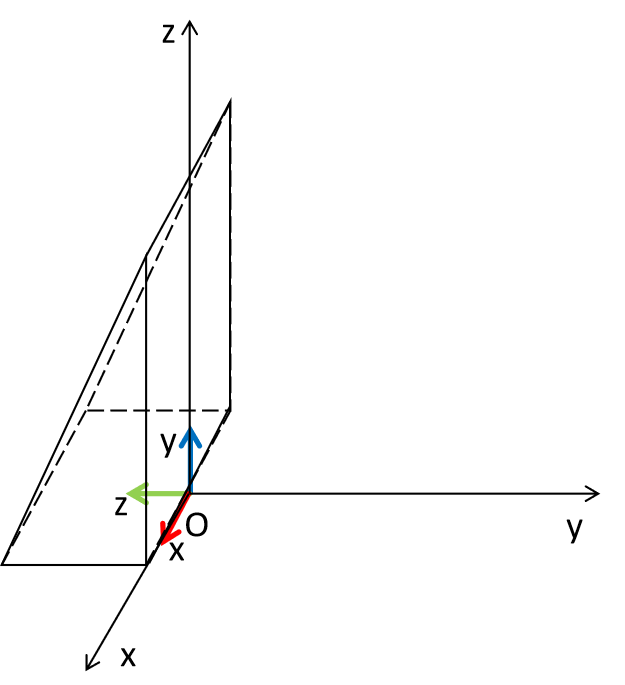
\includegraphics[width=0.95\textwidth]{./figs/Q07_A.png}
        \subcaption{绕$ X_U $轴旋转$ 90^\circ $}
    \end{minipage}
    \begin{minipage}[c]{0.45\textwidth}
        \centering
        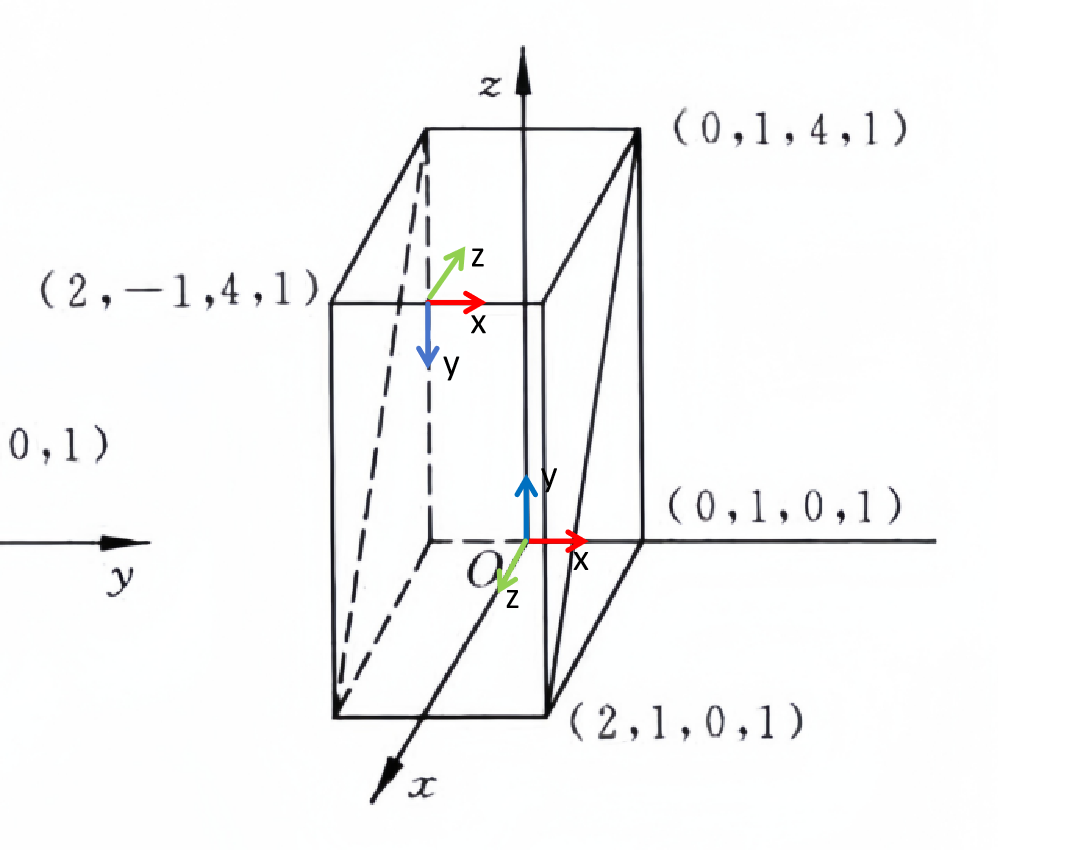
\includegraphics[width=0.95\textwidth]{./figs/Q07_2.png}
        \subcaption{绕$ Z_U $轴旋转$ 90^\circ $}
    \end{minipage}
    \caption{从右至左看A的变换序列}
  \end{figure}

  对于B，
  \begin{figure}
    \centering
    \begin{minipage}[c]{0.45\textwidth}
        \centering
        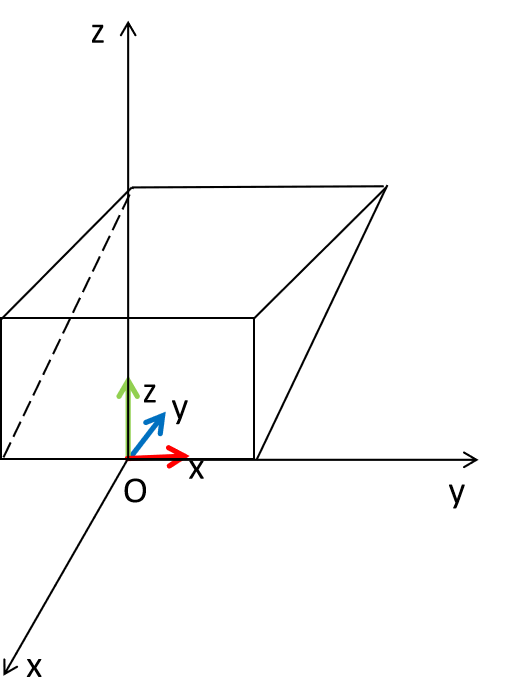
\includegraphics[width=0.95\textwidth]{./figs/Q07_1.png}
        \subcaption{绕$ Z_U $轴旋转$ 90^\circ $}
    \end{minipage}
    \begin{minipage}[c]{0.45\textwidth}
        \centering
        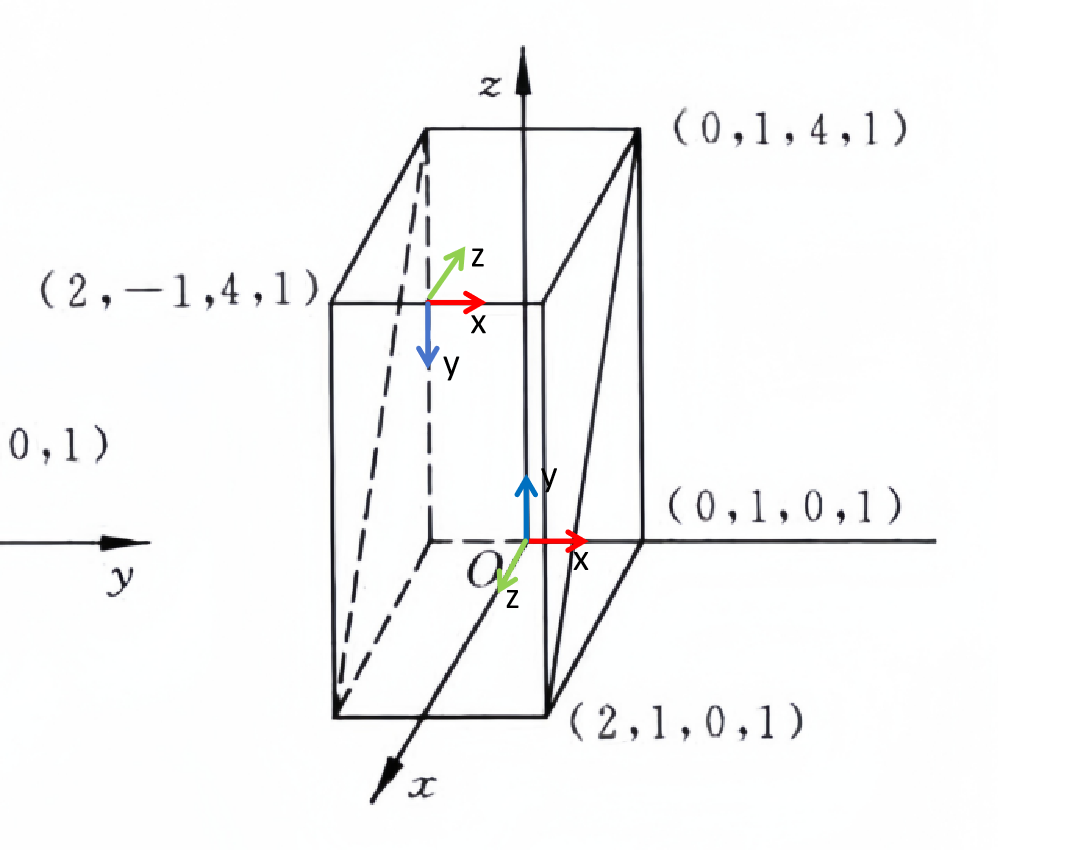
\includegraphics[width=0.95\textwidth]{./figs/Q07_2.png}
        \subcaption{绕$ Y_U $轴旋转$ -90^\circ $}
    \end{minipage}
    \caption{从右至左看B的变换序列}
  \end{figure}

  从左至右看，是以映射的角度看，是相对运动坐标系。

  对于A，
  \begin{figure}
    \centering
    \begin{minipage}[c]{0.45\textwidth}
        \centering
        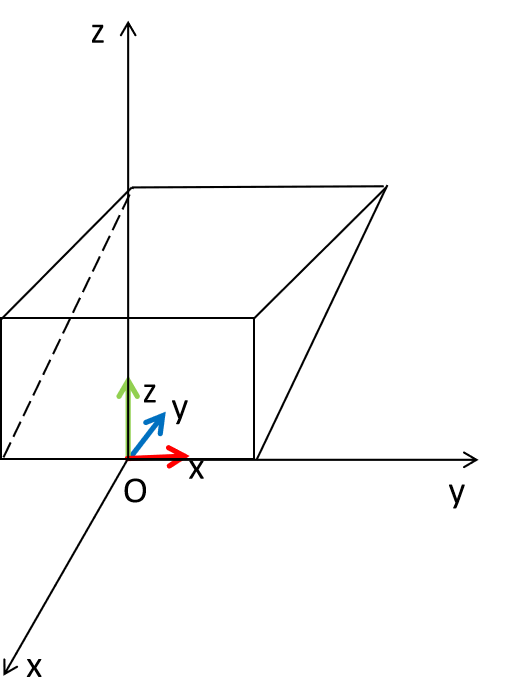
\includegraphics[width=0.95\textwidth]{./figs/Q07_1.png}
        \subcaption{绕$ Z_A $轴旋转$ 90^\circ $}
    \end{minipage}
    \begin{minipage}[c]{0.45\textwidth}
        \centering
        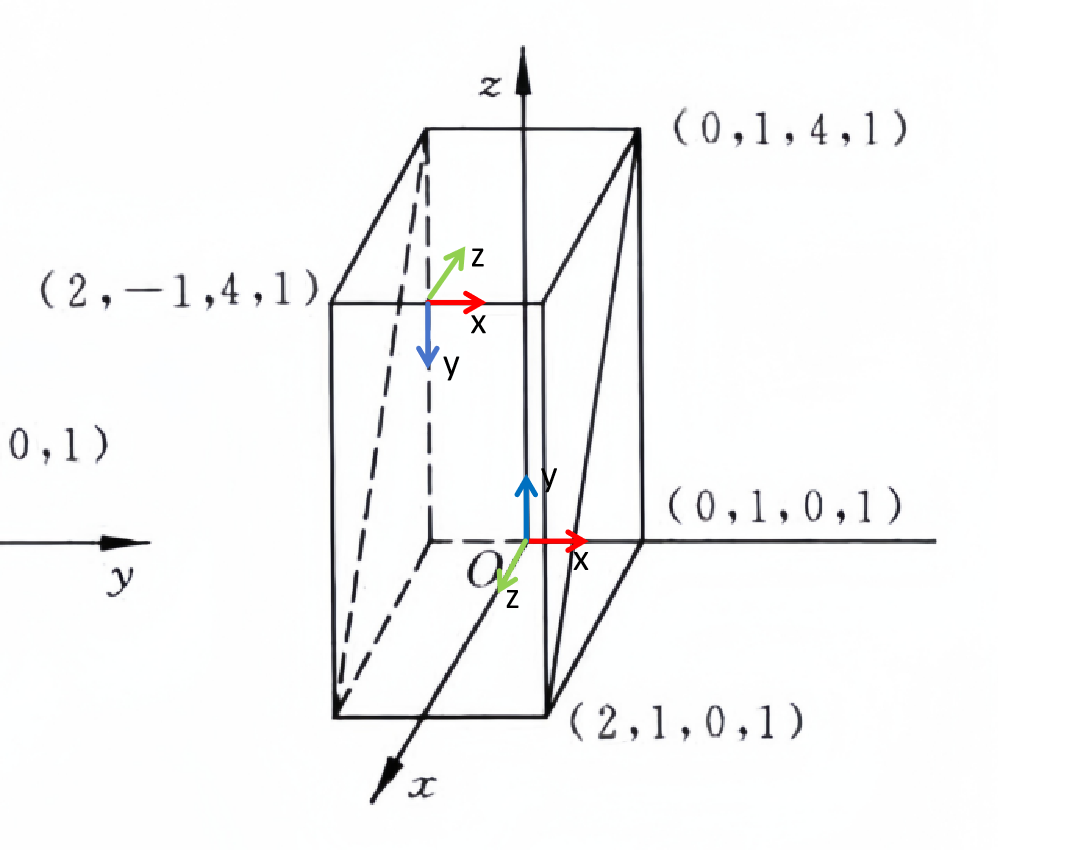
\includegraphics[width=0.95\textwidth]{./figs/Q07_2.png}
        \subcaption{绕$ X_A $轴旋转$ 90^\circ $}
    \end{minipage}
    \caption{从左至右看A的变换序列}
  \end{figure}

  对于B，
  \begin{figure}
    \centering
    \begin{minipage}[c]{0.45\textwidth}
        \centering
        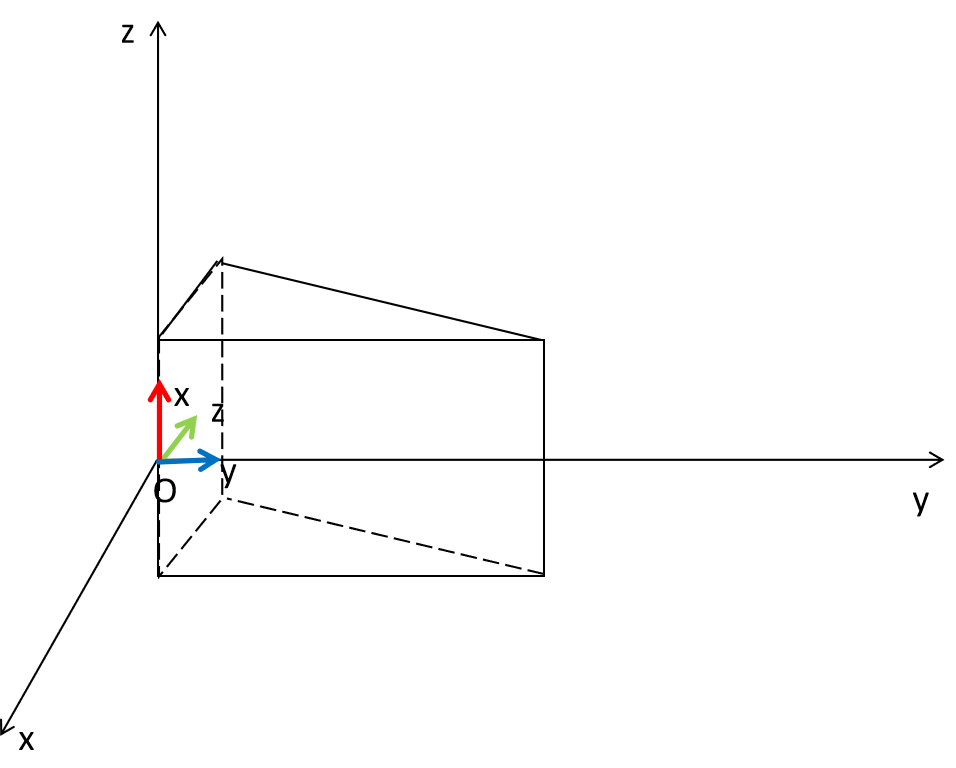
\includegraphics[width=0.95\textwidth]{./figs/Q07_B.png}
        \subcaption{绕$ Y_B $轴旋转$ -90^\circ $}
    \end{minipage}
    \begin{minipage}[c]{0.45\textwidth}
        \centering
        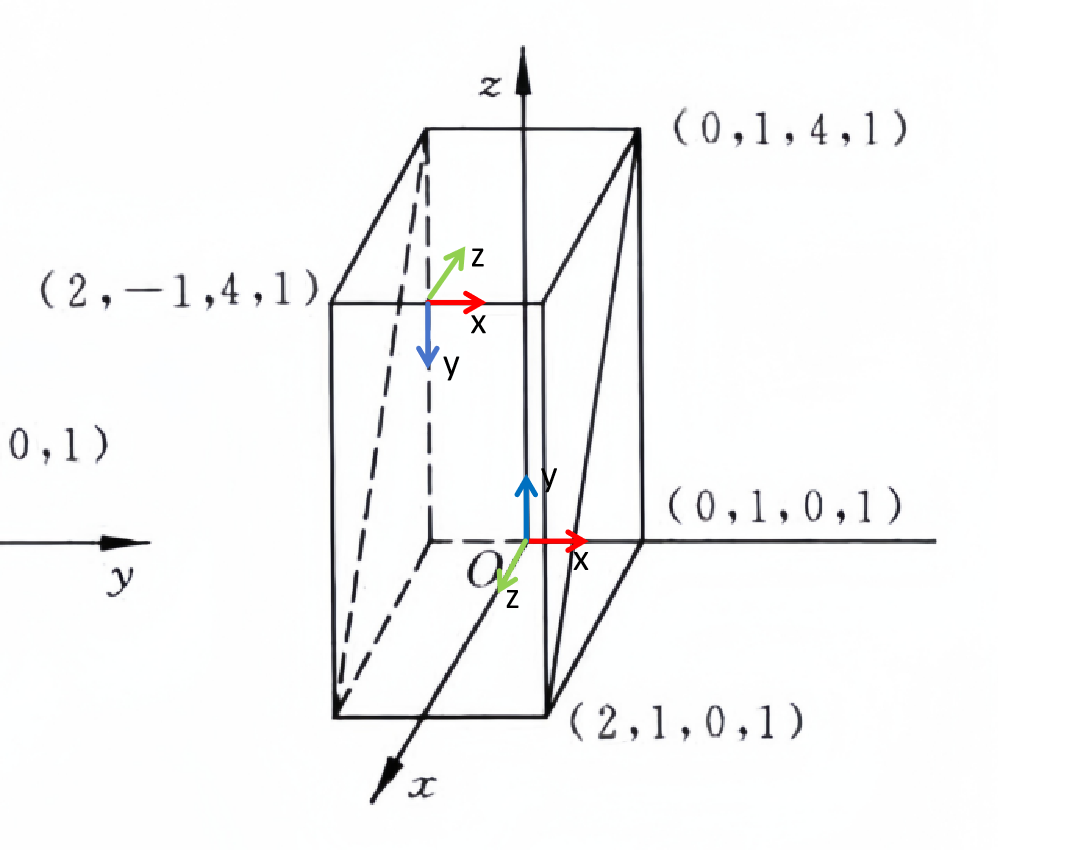
\includegraphics[width=0.95\textwidth]{./figs/Q07_2.png}
        \subcaption{绕$ Z_B $轴旋转$ 90^\circ $}
    \end{minipage}
    \caption{从左至右看B的变换序列}
  \end{figure}

\end{sol}

\question 

\begin{sol}
  由于是固定坐标系，我们以算子的角度来看待。总的旋转矩阵为
  \[
    \mathbf{R} = \mathbf{R}(Z,30^\circ) \mathbf{R}(X,60^\circ)
  \]

  设重复旋转n次之后，点P回到它最初的全局位置。从数学的角度来看，就是对旋转矩阵求n次幂，最后变成了一个单位阵。
  \[
    \mathbf{R}^n = \mathbf{I}
  \]

  我们的任务是求出这个n。
  
  第一种方法，也就是最简单的计算的方法，即直接计算$ \mathbf{R}^2, \mathbf{R}^3 ... $，直到$ \mathbf{R}^n = \mathbf{I} $。

  第二种方法：我们先求出旋转矩阵的特征值$ \lambda_1, \lambda_2, \lambda_3 $，然后分别求出使得$ \lambda^k = 1 $的k值，求出这3个k值的最小公倍数，即为n。

  第三种方法，是将旋转矩阵等效为绕某个K轴旋转$\theta$。然后计算
  \[
    \theta \cdot n = 2 \pi k
  \]

  于是
  \[
    n = \frac{2 \pi k}{\theta}
  \]

  在使用计算机程序实际计算的过程中，发现设置的tolerance（由于计算机使用浮点数计算，所以需要设置一个很小的浮点数作为容忍度）对结果的影响很大。在设置$ tolerance = 10^{-4} $时，得到计算结果$ n = 16637 $。
  
\end{sol}

\question 

\begin{sol}
  先计算5个单位时间后的$ ^B\mathbf{p} $。
  \[
    ^B\mathbf{p} = ^B\mathbf{p}_0 + ^B\mathbf{V}_0 \cdot t
  \]

  再将$ ^B\mathbf{p} $转换为$ ^A\mathbf{p} $。
  \[
    ^A\mathbf{p} = _B^A\mathbf{T} ^B\mathbf{p}
  \]

  注意这里需要将$ ^B\mathbf{p} $转换为齐次坐标的形式再计算。
  \[
    ^A\mathbf{p} = \begin{pmatrix} -14.4184 & 14.7971 & -8.7715 \end{pmatrix}^T
  \]
  
\end{sol}

\question 

\begin{sol}
  \[
    \mathbf{T}^{-1} =
    \begin{bmatrix}
      0 & 0 & -1 & 3 \\
      1 & 0 & 0 & 1 \\
      0 & -1 & 0 & 2 \\
      0 & 0 & 0 & 1
    \end{bmatrix}
  \]
  
\end{sol}

\question 

\begin{sol}
  对于问题a
  \[
    _B^A\mathbf{R} = \begin{pmatrix} ^A\mathbf{X}_B & ^A\mathbf{Y}_B & ^A\mathbf{Z}_B \end{pmatrix} = 
    \begin{bmatrix}
      1 & 0 & 0 \\
      0 & 0 & 1 \\
      0 & -1 & 0 
    \end{bmatrix}
  \]

  对于问题b
  \begin{align*}
    \alpha = 90^\circ \\
    \beta = 90^\circ \\
    \gamma = -90^\circ
  \end{align*}
  
\end{sol}

\question 

\begin{sol}
  对于问题a，旋转矩阵需要满足的条件是：它是个正交矩阵，且行列式等于1。用数学的语言表达是
  \begin{align*}
    _B^A\mathbf{R} _B^A\mathbf{R}^T = I \\
    det(_B^A\mathbf{R}) = 1
  \end{align*}

  经检查，$ _B^A\mathbf{R} $是旋转变换。

  问题b和问题c其实问的是一个问题
  \begin{align*}
    & yaw = 0^\circ \\
    & pitch = 58.2117^\circ \\
    & roll = 278.8538^\circ
  \end{align*}
  
\end{sol}

\question 

\begin{sol}
  我们假设这个轴为z轴（因为坐标变换不影响一般性），则旋转变换$ R(Z, \theta) = 
  \begin{bmatrix}
    \cos\theta & -\sin\theta & 0 \\
    \sin\theta & \cos\theta & 0 \\
    0 & 0 & 1
  \end{bmatrix} $，对应的齐次变换矩阵为$
  \begin{bmatrix}
    \cos\theta & -\sin\theta & 0 & 0 \\
    \sin\theta & \cos\theta & 0 & 0 \\
    0 & 0 & 1 & 0 \\
    0 & 0 & 0 & 1 
  \end{bmatrix} $；平移变换$ Q = \begin{pmatrix} 0 & 0 & d \end{pmatrix} $，对应的齐次变换矩阵为$
  \begin{bmatrix}
    1 & 0 & 0 & 0 \\
    0 & 1 & 0 & 0 \\
    0 & 0 & 1 & d \\
    0 & 0 & 0 & 1 
  \end{bmatrix} $。

  先旋转后移动对应的齐次变换矩阵为
  \[
    \begin{bmatrix}
      \cos\theta & -\sin\theta & 0 & 0 \\
      \sin\theta & \cos\theta & 0 & 0 \\
      0 & 0 & 1 & 0 \\
      0 & 0 & 0 & 1 
    \end{bmatrix}
    \begin{bmatrix}
      1 & 0 & 0 & 0 \\
      0 & 1 & 0 & 0 \\
      0 & 0 & 1 & d \\
      0 & 0 & 0 & 1 
    \end{bmatrix}
    =
    \begin{bmatrix}
      \cos\theta & -\sin\theta & 0 & 0 \\
      \sin\theta & \cos\theta & 0 & 0 \\
      0 & 0 & 1 & d \\
      0 & 0 & 0 & 1 
    \end{bmatrix}
  \]

  先平移后旋转对应的齐次变换矩阵为
  \[
    \begin{bmatrix}
      1 & 0 & 0 & 0 \\
      0 & 1 & 0 & 0 \\
      0 & 0 & 1 & d \\
      0 & 0 & 0 & 1 
    \end{bmatrix}
    \begin{bmatrix}
      \cos\theta & -\sin\theta & 0 & 0 \\
      \sin\theta & \cos\theta & 0 & 0 \\
      0 & 0 & 1 & 0 \\
      0 & 0 & 0 & 1 
    \end{bmatrix}
    =
    \begin{bmatrix}
      \cos\theta & -\sin\theta & 0 & 0 \\
      \sin\theta & \cos\theta & 0 & 0 \\
      0 & 0 & 1 & d \\
      0 & 0 & 0 & 1 
    \end{bmatrix}
  \]

  两种顺序得到相同结果，因此，绕某轴的旋转变换与沿同一轴的移动变换的次序可交换。

  两次不同的平移对应的齐次变换矩阵为
  \[
    \begin{bmatrix}
      1 & 0 & 0 & 0 \\
      0 & 1 & 0 & 0 \\
      0 & 0 & 1 & d_1 \\
      0 & 0 & 0 & 1 
    \end{bmatrix}
    \begin{bmatrix}
      1 & 0 & 0 & 0 \\
      0 & 1 & 0 & 0 \\
      0 & 0 & 1 & d_2 \\
      0 & 0 & 0 & 1 
    \end{bmatrix}
    =
    \begin{bmatrix}
      1 & 0 & 0 & 0 \\
      0 & 1 & 0 & 0 \\
      0 & 0 & 1 & d_1 + d_2 \\
      0 & 0 & 0 & 1 
    \end{bmatrix}
  \]

  \[
    \begin{bmatrix}
      1 & 0 & 0 & 0 \\
      0 & 1 & 0 & 0 \\
      0 & 0 & 1 & d_2 \\
      0 & 0 & 0 & 1 
    \end{bmatrix}
    \begin{bmatrix}
      1 & 0 & 0 & 0 \\
      0 & 1 & 0 & 0 \\
      0 & 0 & 1 & d_1 \\
      0 & 0 & 0 & 1 
    \end{bmatrix}
    =
    \begin{bmatrix}
      1 & 0 & 0 & 0 \\
      0 & 1 & 0 & 0 \\
      0 & 0 & 1 & d_1 + d_2 \\
      0 & 0 & 0 & 1 
    \end{bmatrix} 
  \]

  两种顺序得到相同结果，因此，两沿同一轴的移动变换的次序可交换。

  两次不同的旋转对应的齐次变换矩阵为
  \[
    \begin{bmatrix}
      \cos\theta_1 & -\sin\theta_1 & 0 & 0 \\
      \sin\theta_1 & \cos\theta_1 & 0 & 0 \\
      0 & 0 & 1 & 0 \\
      0 & 0 & 0 & 1 
    \end{bmatrix}
    \begin{bmatrix}
      \cos\theta_2 & -\sin\theta_2 & 0 & 0 \\
      \sin\theta_2 & \cos\theta_2 & 0 & 0 \\
      0 & 0 & 1 & 0 \\
      0 & 0 & 0 & 1 
    \end{bmatrix}
    =
    \begin{bmatrix}
      \cos(\theta_1 + \theta_2) & -\sin(\theta_1 + \theta_2) & 0 & 0 \\
      \sin(\theta_1 + \theta_2) & \cos(\theta_1 + \theta_2) & 0 & 0 \\
      0 & 0 & 1 & 0 \\
      0 & 0 & 0 & 1  
    \end{bmatrix}
  \]

  \[
    \begin{bmatrix}
      \cos\theta_2 & -\sin\theta_2 & 0 & 0 \\
      \sin\theta_2 & \cos\theta_2 & 0 & 0 \\
      0 & 0 & 1 & 0 \\
      0 & 0 & 0 & 1
    \end{bmatrix}
    \begin{bmatrix}
      \cos\theta_1 & -\sin\theta_1 & 0 & 0 \\
      \sin\theta_1 & \cos\theta_1 & 0 & 0 \\
      0 & 0 & 1 & 0 \\
      0 & 0 & 0 & 1
    \end{bmatrix}
    =
    \begin{bmatrix}
      \cos(\theta_1 + \theta_2) & -\sin(\theta_1 + \theta_2) & 0 & 0 \\
      \sin(\theta_1 + \theta_2) & \cos(\theta_1 + \theta_2) & 0 & 0 \\
      0 & 0 & 1 & 0 \\
      0 & 0 & 0 & 1  
    \end{bmatrix} 
  \]

  两种顺序得到相同结果，因此，两同轴的旋转变换的次序可交换。
  
\end{sol}

\question 

\begin{sol}
  添加辅助坐标系{A'}和{B'}，其中{A'}与{A}固连，{B'}与{B}固连，{A'}和{B'}的Z轴与$ \mathbf{k} $重合，且在旋转之前{B'}和{A'}重合，{B}和{A}重合。因此有：
  \[
    _{A'}^A\mathbf{R} = _{B'}^B\mathbf{R} = 
    \begin{bmatrix}
      n_x & o_x & k_x \\
      n_y & o_y & k_y \\
      n_z & o_z & k_z
    \end{bmatrix}
  \]

  坐标系{B}绕$ \mathbf{k} $相对{A}旋转$ \theta $角，相当于坐标系{B'}相对{A'}的Z轴旋转$ \theta $角，保持其它关系不变，则有
  \[
    \mathbf{R}(\mathbf{k}, \theta) = _{B}^A\mathbf{R} = _{A'}^A\mathbf{R} _{B'}^{A'}\mathbf{R} _{B}^{B'}\mathbf{R}
  \]

  由于$ _{B}^{B'}\mathbf{R} = _{B'}^{B}\mathbf{R}^{-1} = _{B'}^{B}\mathbf{R}^T $，且$ _{B'}^{A'}\mathbf{R} = \mathbf{R}(Z, \theta) $，因此
  \[
    \mathbf{R}(\mathbf{k}, \theta) = _{A'}^A\mathbf{R} R(Z, \theta) _{B'}^{B}\mathbf{R}^T
  \]

  即
  \[
    \mathbf{R}(\mathbf{k}, \theta) = 
    \begin{bmatrix}
      n_x & o_x & k_x \\
      n_y & o_y & k_y \\
      n_z & o_z & k_z
    \end{bmatrix}
    \begin{bmatrix}
      \cos\theta & -\sin\theta & 0 \\
      \sin\theta & \cos\theta & 0 \\
      0 & 0 & 1
    \end{bmatrix}
    \begin{bmatrix}
      n_x & n_y & n_z \\
      o_x & o_y & o_z \\
      k_x & k_y & k_z
    \end{bmatrix}
  \]

  经计算，得到
  \begingroup
  \small
  \[ 
    \begin{bmatrix}
      k_x^2 + (o_x^2 + n_x^2)c\theta & k_x k_y + (n_x n_y + o_x o_y)c\theta - (n_x o_y - o_x n_y)s\theta & k_x k_z + (n_x n_z + o_x o_z)c\theta - (n_x o_z - o_x n_z)s\theta \\
      k_x k_y + (n_x n_y + o_x o_y)c\theta + (n_x o_y - o_x n_y)s\theta & k_y^2 + (n_y^2 + o_y^2)c\theta & k_y k_z + (n_y n_z + o_y o_z)c\theta - (n_y o_z - o_y n_z)s\theta \\
      k_x k_z + (n_x n_z + o_x o_z)c\theta + (n_x o_z - o_x n_z)s\theta & k_y k_z + (n_y n_z + o_y o_z)c\theta + (n_y o_z - o_y n_z)s\theta & k_z^2 + (o_z^2 + n_z^2)c\theta
    \end{bmatrix}
  \]
  \endgroup

  这个式子是可以化简的。首先，因为$ _{B}^{B'}\mathbf{R} = _{B'}^{B}\mathbf{R}^T $是一个正交矩阵，它的3个列矢量都是单位矢量，且相互正交。所以
  \begin{align*}
    & n_x^2 + o_x^2 + k_x^2 = 1 \\
    & n_y^2 + o_y^2 + k_y^2 = 1 \\
    & n_z^2 + o_z^2 + k_z^2 = 1 \\
    & n_x n_y + o_x o_y + k_x k_y = 0 \\
    & n_x n_z + o_x o_z + k_x k_z = 0 \\
    & n_y n_z + o_y o_z + k_y k_z = 0 
  \end{align*}

  因此
  \begin{align*}
    & n_x^2 + o_x^2 = 1 - k_x^2 \\
    & n_y^2 + o_y^2 = 1 - k_y^2 \\
    & n_z^2 + o_z^2 = 1 - k_z^2 \\
    & n_x n_y + o_x o_y = -k_x k_y \\
    & n_x n_z + o_x o_z = -k_x k_z \\
    & n_y n_z + o_y o_z = -k_y k_z 
  \end{align*}

  接下来我们要先证明一个引理：旋转矩阵中每一个元素的值都与它的代数余子式的值相等。

  证明过程如下：旋转矩阵是正交矩阵，所以$ R^{-1} = R^T $。而采用一般的求逆矩阵的方法，$ R^{-1} = \frac{1}{det(R)} R^* $。而$ det(R) = 1 $，所以$ R^{-1} = R^* $，因此$ R^T = R^* $。又因为$ R^* = (R_{ji}) $，其中$ R_{ji} $是元素$ r_{ji} $的代数余子式。因此我们得到$ R^T = (R_{ji}) $，也就是$ R = (R_{ij}) $。引理得证。
  
  运用这个引理，我们可以得到如下式子：
  \[
    k_x = -
    \begin{vmatrix}
      n_y & n_z \\
      o_y & o_z 
    \end{vmatrix}
    = n_y o_z - o_y n_z 
  \]
  
  \[
    k_y = -
    \begin{vmatrix}
      n_x & n_z \\
      o_x & o_z 
    \end{vmatrix}
    = -(n_x o_z - o_x n_z)
  \] 

  \[
    k_z = 
    \begin{vmatrix}
      n_x & n_y \\
      o_x & o_y 
    \end{vmatrix}
    = n_x o_y - o_x n_y
  \]

  将上面得到的9个式子代入我们之前计算得到的矩阵，我们得到最终的结果
  \[ 
    \begin{bmatrix}
      k_x k_x v\theta + c\theta & k_x k_y v\theta - k_zs\theta & k_x k_z v\theta + k_ys\theta \\
      k_x k_y v\theta + k_zs\theta & k_y k_y v\theta + c\theta & k_y k_z v\theta - k_xs\theta \\
      k_x k_z v\theta - k_ys\theta & k_y k_z v\theta + k_xs\theta & k_z k_z v\theta + c\theta
    \end{bmatrix}
  \]
  
\end{sol}

\question 

\begin{sol}
  由于$ \theta $足够小，所以$ \sin\theta = \theta, \cos\theta = 1 $，代入上一题的结果，得
  \[ 
    R(\mathbf{k}, \theta) = 
    \begin{bmatrix}
      1 & -k_z\theta & k_y\theta \\
      k_z\theta & 1 & -k_x\theta \\
      -k_y\theta & k_x\theta & 1
    \end{bmatrix}
    = \mathbf{I} + \theta [\mathbf{k}]
  \]
  其中$ [\mathbf{k}] $是向量$ \mathbf{k} $的叉乘矩阵。

  考虑两个无穷小旋转：
  \begin{itemize}
    \item 绕轴$ \mathbf{k}_1 $旋转$ \theta_1 $，旋转矩阵为$ \mathbf{R}_1 = \mathbf{I} + \theta_1 [\mathbf{k}_1] $
    \item 绕轴$ \mathbf{k}_2 $旋转$ \theta_2 $，旋转矩阵为$ \mathbf{R}_2 = \mathbf{I} + \theta_2 [\mathbf{k}_2] $
  \end{itemize}

  先旋转1后旋转2
  \[ 
    \mathbf{R}_2 \mathbf{R}_1 = (\mathbf{I} + \theta_2 [\mathbf{k}_2])(\mathbf{I} + \theta_1 [\mathbf{k}_1]) = \mathbf{I} + \theta_1 [\mathbf{k}_1] + \theta_2 [\mathbf{k}_2] + \theta_1 \theta_2 [\mathbf{k}_2] [\mathbf{k}_1]
  \]

  由于$ \theta $是无穷小量，所以它们的乘积$ \theta_1 \theta_2 $可以忽略，因此
  \[ 
    \mathbf{R}_2 \mathbf{R}_1 \approx \mathbf{I} + \theta_1 [\mathbf{k}_1] + \theta_2 [\mathbf{k}_2]
  \]

  先旋转2后旋转1
  \[ 
    \mathbf{R}_1 \mathbf{R}_2 = (\mathbf{I} + \theta_1 [\mathbf{k}_1])(\mathbf{I} + \theta_2 [\mathbf{k}_2]) = \mathbf{I} + \theta_1 [\mathbf{k}_1] + \theta_2 [\mathbf{k}_2] + \theta_1 \theta_2 [\mathbf{k}_1] [\mathbf{k}_2] \approx \mathbf{I} + \theta_1 [\mathbf{k}_1] + \theta_2 [\mathbf{k}_2]
  \]

  两者相等，故$ \mathbf{R}_2 \mathbf{R}_1 = \mathbf{R}_1 \mathbf{R}_2 $，即两个无穷小旋转相乘可交换。
  
\end{sol}

\question 

\begin{sol}
  一般轴旋转的等效旋转矩阵其实还可以写成如下的形式：
  \[ 
    \mathbf{R}(\mathbf{f}, \theta) = \mathbf{I} + \sin\theta [\mathbf{f}] + (1 - \cos\theta) [\mathbf{f}]^2
  \]
  其中$ [\mathbf{f}] = 
  \begin{bmatrix}
    0 & -f_z & f_y \\
    f_z & 0 & -f_x \\
    -f_y & f_x & 0
  \end{bmatrix} $是向量$ \mathbf{f} $的叉乘矩阵。

  现在，考虑矩阵指数$ e^{[\mathbf{f}]\theta} $，由泰勒公式得，
  \[ 
    e^{[\mathbf{f}]\theta} = \mathbf{I} + [\mathbf{f}]\theta + \frac{([\mathbf{f}]\theta)^2}{2!} + \frac{([\mathbf{f}]\theta)^3}{3!} + \frac{([\mathbf{f}]\theta)^4}{4!} + \dots
  \]

  由于$ \mathbf{f} $是斜对称矩阵，且对于单位矢量，有$ [\mathbf{f}]^3 = -[\mathbf{f}], [\mathbf{f}]^4 = -[\mathbf{f}]^2, [\mathbf{f}]^5 = [\mathbf{f}] $等性质，代入级数
  \[ 
    e^{[\mathbf{f}]\theta} = \mathbf{I} + [\mathbf{f}]\theta + \frac{\theta^2}{2!} [\mathbf{f}]^2 + \frac{\theta^3}{3!}(-[\mathbf{f}]) + \frac{\theta^4}{4!}(-[\mathbf{f}]^2) + \frac{\theta^5}{5!}[\mathbf{f}] + \frac{\theta^6}{6!}[\mathbf{f}]^2 + \dots
  \]

  重新分组项，得
  \[ 
    e^{[\mathbf{f}]\theta} = \mathbf{I} + (\theta - \frac{\theta^3}{3!} + \frac{\theta^5}{5!} - \dots)[\mathbf{f}] + (\frac{\theta^2}{2!} - \frac{\theta^4}{4!} + \frac{\theta^6}{6!} - \dots)[\mathbf{f}]^2
  \]

  又由于
  \begin{align*}
    & \theta - \frac{\theta^3}{3!} + \frac{\theta^5}{5!} - \dots = \sin\theta \\
    & \frac{\theta^2}{2!} - \frac{\theta^4}{4!} + \frac{\theta^6}{6!} - \dots = 1 - \cos\theta
  \end{align*}

  因此
  \[ 
    e^{[\mathbf{f}]\theta} = \mathbf{I} + \sin\theta[\mathbf{f}] + (1 - \cos\theta)[\mathbf{f}]^2
  \]

  所以
  \[ 
    \mathbf{R}(\mathbf{f}, \theta) = e^{[\mathbf{f}]\theta} 
  \]
\end{sol}

\question 

\begin{sol}
  对于方程
  \[
    k_1 {^G}\mathbf{X}_B + k_2 {^G}\mathbf{Y}_B + k_3 {^G}\mathbf{Z}_B = 0
  \]

  两边同时点乘$ {^G}\mathbf{X}_B $，得到
  \[
    k_1({^G}\mathbf{X}_B \cdot {^G}\mathbf{X}_B) + k_2({^G}\mathbf{Y}_B \cdot {^G}\mathbf{X}_B) + k_3({^G}\mathbf{Z}_B \cdot {^G}\mathbf{X}_B) = 0
  \]

  由于坐标系的轴之间相互正交，即$ {^G}\mathbf{Y}_B \cdot {^G}\mathbf{X}_B = 0, {^G}\mathbf{Z}_B \cdot {^G}\mathbf{X}_B = 0 $，所以$ k_1 = 0 $。

  同时点乘$ {^G}\mathbf{Y}_B $和$ {^G}\mathbf{Z}_B $，也可以得到$ k_2 = 0 $和$ k_3 = 0 $。因此方程$ k_1 {^G}\mathbf{X}_B + k_2 {^G}\mathbf{Y}_B + k_3 {^G}\mathbf{Z}_B = 0 $仅有唯一解$ k_1 = k_2 = k_3 = 0 $，这证明刚体坐标系B的单位矢量在全局坐标系G中是线性独立的。
  
\end{sol}

\question 

\begin{sol}
  设正交矩阵$ \mathbf{R}_1, \mathbf{R}_2 $。它们的乘积为$ \mathbf{R} $。要证明$ \mathbf{R} $为正交矩阵，即证明$ \mathbf{R} \mathbf{R}^T = \mathbf{I} $。

  将$ \mathbf{R} = \mathbf{R}_1 \mathbf{R}_2 $代入，得
  \[
    (\mathbf{R}_1 \mathbf{R}_2)(\mathbf{R}_1 \mathbf{R}_2)^T = \mathbf{I}
  \]

  由矩阵转置的性质，可以得到
  \[
    \mathbf{R}_1 \mathbf{R}_2 \mathbf{R}_2^T \mathbf{R}_1^T = \mathbf{I}
  \]

  由于$ \mathbf{R}_1, \mathbf{R}_2 $均为正交矩阵，即$ \mathbf{R}_1 \mathbf{R}_1^T = \mathbf{I}, \mathbf{R}_2 \mathbf{R}_2^T = \mathbf{I} $。得证。
  
\end{sol}

\question 

\begin{sol}
  设
  \begin{align*}
    \mathbf{a} = (a_1, a_2, a_3) \\
    \mathbf{b} = (b_1, b_2, b_3)
  \end{align*}
  旋转矩阵
  \[
    \mathbf{R} = 
    \begin{bmatrix}
      r_{11} & r_{12} & r_{13} \\
      r_{21} & r_{22} & r_{23} \\
      r_{31} & r_{32} & r_{33}
    \end{bmatrix}
  \]

  根据叉积的定义，
  \[
    \mathbf{a} \times \mathbf{b} = 
    \begin{vmatrix}
      \mathbf{i} & \mathbf{j} & \mathbf{k} \\
      a_1 & a_2 & a_3 \\
      b_1 & b_2 & b_3
    \end{vmatrix}
    = 
    \begin{pmatrix}  
      a_2 b_3 - a_3 b_2 \\
      a_3 b_1 - a_1 b_3 \\
      a_1 b_2 - a_2 b_1
    \end{pmatrix}
  \]

  所以
  \[
    \mathbf{R} (\mathbf{a} \times \mathbf{b})= 
    \begin{bmatrix}
      r_{11} & r_{12} & r_{13} \\
      r_{21} & r_{22} & r_{23} \\
      r_{31} & r_{32} & r_{33}
    \end{bmatrix}
    \begin{pmatrix}  
      a_2 b_3 - a_3 b_2 \\
      a_3 b_1 - a_1 b_3 \\
      a_1 b_2 - a_2 b_1
    \end{pmatrix}
    =
    \begin{pmatrix}  
      r_{11} a_2 b_3 - r_{11} a_3 b_2 + r_{12} a_3 b_1 - r_{12} a_1 b_3 + r_{13} a_1 b_2 - r_{13} a_2 b_1 \\
      r_{21} a_2 b_3 - r_{21} a_3 b_2 + r_{22} a_3 b_1 - r_{22} a_1 b_3 + r_{23} a_1 b_2 - r_{23} a_2 b_1 \\
      r_{31} a_2 b_3 - r_{31} a_3 b_2 + r_{32} a_3 b_1 - r_{32} a_1 b_3 + r_{33} a_1 b_2 - r_{33} a_2 b_1
    \end{pmatrix}
  \]

  \[
    \mathbf{R} \mathbf{a} = 
    \begin{bmatrix}
      r_{11} & r_{12} & r_{13} \\
      r_{21} & r_{22} & r_{23} \\
      r_{31} & r_{32} & r_{33}
    \end{bmatrix}
    \begin{pmatrix}  
      a_1 \\
      a_2 \\
      a_3
    \end{pmatrix}
    =
    \begin{pmatrix}  
      r_{11} a_1 + r_{12} a_2 + r_{13} a_3 \\
      r_{21} a_1 + r_{22} a_2 + r_{23} a_3 \\
      r_{31} a_1 + r_{32} a_2 + r_{33} a_3 
    \end{pmatrix}
  \]

  同理，
  \[
    \mathbf{R} \mathbf{b} = 
    \begin{bmatrix}
      r_{11} & r_{12} & r_{13} \\
      r_{21} & r_{22} & r_{23} \\
      r_{31} & r_{32} & r_{33}
    \end{bmatrix}
    \begin{pmatrix}  
      b_1 \\
      b_2 \\
      b_3
    \end{pmatrix}
    =
    \begin{pmatrix}  
      r_{11} b_1 + r_{12} b_2 + r_{13} b_3 \\
      r_{21} b_1 + r_{22} b_2 + r_{23} b_3 \\
      r_{31} b_1 + r_{32} b_2 + r_{33} b_3 
    \end{pmatrix}
  \]

  所以，
  \[
    \mathbf{R} \mathbf{a} \times \mathbf{R} \mathbf{b} = 
    \begin{vmatrix}
      \mathbf{i} & \mathbf{j} & \mathbf{k} \\
      r_{11} a_1 + r_{12} a_2 + r_{13} a_3 & r_{21} a_1 + r_{22} a_2 + r_{23} a_3 & r_{31} a_1 + r_{32} a_2 + r_{33} a_3 \\
      r_{11} b_1 + r_{12} b_2 + r_{13} b_3 & r_{21} b_1 + r_{22} b_2 + r_{23} b_3 & r_{31} b_1 + r_{32} b_2 + r_{33} b_3
    \end{vmatrix}
  \]

  即
  \[
    \begin{pmatrix}  
      (r_{21} a_1 + r_{22} a_2 + r_{23} a_3)(r_{31} b_1 + r_{32} b_2 + r_{33} b_3) - (r_{21} b_1 + r_{22} b_2 + r_{23} b_3)(r_{31} a_1 + r_{32} a_2 + r_{33} a_3) \\
      (r_{31} a_1 + r_{32} a_2 + r_{33} a_3)(r_{11} b_1 + r_{12} b_2 + r_{13} b_3) - (r_{11} a_1 + r_{12} a_2 + r_{13} a_3)(r_{31} b_1 + r_{32} b_2 + r_{33} b_3) \\
      (r_{11} a_1 + r_{12} a_2 + r_{13} a_3)(r_{21} b_1 + r_{22} b_2 + r_{23} b_3) - (r_{21} a_1 + r_{22} a_2 + r_{23} a_3)(r_{11} b_1 + r_{12} b_2 + r_{13} b_3)
    \end{pmatrix}
  \]

  化简后得到
  \begingroup
  \small
  \[
    \begin{pmatrix}  
      (r_{21} r_{32} - r_{31} r_{22}) a_1 b_2 + (r_{21} r_{33} - r_{31} r_{23}) a_1 b_3 + (r_{22} r_{31} - r_{32} r_{21}) a_2 b_1 +(r_{22} r_{33} - r_{32} r_{23}) a_2 b_3 + (r_{31} r_{23} - r_{21} r_{33}) a_3 b_1 + (r_{32} r_{23} - r_{22} r_{33}) a_3 b_2 \\
      \dots \\
      \dots 
    \end{pmatrix}
  \]
  \endgroup
  
  由于计算量过大，我们只写出了向量的第一个元素，剩下两个元素应该和第一个同理。我们可以看到，这个式子和之前求出的似乎很不一样，我们对比一下
  \begin{align*}
    r_{11} = r_{22} r_{33} - r_{32} r_{23} \\
    r_{12} = r_{31} r_{23} - r_{21} r_{33} \\
    r_{13} = r_{21} r_{32} - r_{31} r_{22}
  \end{align*}

  这些式子可以变成行列式的形式
  \[
    r_{11} = 
    \begin{vmatrix}
      r_{22} & r_{23} \\
      r_{32} & r_{33}
    \end{vmatrix} 
  \]

  \[
    r_{12} = -
    \begin{vmatrix}
      r_{21} & r_{23} \\
      r_{31} & r_{33}
    \end{vmatrix} 
  \]

  \[
    r_{13} = 
    \begin{vmatrix}
      r_{21} & r_{22} \\
      r_{31} & r_{32}
    \end{vmatrix} 
  \]

  由于我们之前在问题14中已经证明引理：旋转矩阵中每一个元素的值都与它的代数余子式的值相等，于是这些式子成立。

  我们证明了等式左右两边的运算结果相等，自然就证明了命题成立。
  
\end{sol}

\question 

\begin{sol}
  设
  \begin{align*}
    \mathbf{a} = (a_1, a_2, a_3) \\
    \mathbf{b} = (b_1, b_2, b_3) \\
    \mathbf{c} = (c_1, c_2, c_3)
  \end{align*}

  根据叉积的定义，
  \[
    \mathbf{b} \times \mathbf{c} = 
    \begin{vmatrix}
      \mathbf{i} & \mathbf{j} & \mathbf{k} \\
      b_1 & b_2 & b_3 \\
      c_1 & c_2 & c_3
    \end{vmatrix}
    = (b_2 c_3 - b_3 c_2, b_3 c_1 - b_1 c_3, b_1 c_2 - b_2 c_1)
  \]

  所以
  \[
    \mathbf{a} \cdot (\mathbf{b} \times \mathbf{c}) = a_1(b_2 c_3 - b_3 c_2) + a_2(b_3 c_1 - b_1 c_3) + a_3(b_1 c_2 - b_2 c_1) = a_1 b_2 c_3 - a_1 b_3 c_2 + a_2 b_3 c_1 - a_2 b_1 c_3 + a_3 b_1 c_2 - a_3 b_2 c_1
  \]

  同理，
  \[
    \mathbf{a} \times \mathbf{b} = 
    \begin{vmatrix}
      \mathbf{i} & \mathbf{j} & \mathbf{k} \\
      a_1 & a_2 & a_3 \\
      b_1 & b_2 & b_3
    \end{vmatrix}
    = (a_2 b_3 - a_3 b_2, a_3 b_1 - a_1 b_3, a_1 b_2 - a_2 b_1)
  \]

  \[
    (\mathbf{a} \times \mathbf{b}) \cdot \mathbf{c} = (a_2 b_3 - a_3 b_2)c_1 + (a_3 b_1 - a_1 b_3)c_2 + (a_1 b_2 - a_2 b_1)c_3 = a_2 b_3 c_1 - a_3 b_2 c_1 + a_3 b_1 c_2 - a_1 b_3 c_2 + a_1 b_2 c_3 - a_2 b_1 c_3 
  \]

  结果完全一致，因此得证。
  
\end{sol}

\question 

\begin{sol}
  我们观察一下点P旋转前和旋转后的坐标，发现这个坐标被循环移位了，所以我们推断旋转矩阵应该是这样的
  \[
  _B^A\mathbf{R} =
    \begin{bmatrix}
      0 & 0 & 1 \\
      1 & 0 & 0 \\
      0 & 1 & 0
    \end{bmatrix}
  \]

  我们画出坐标系示意图，发现坐标系{B}的x轴就是坐标系{A}的y轴，坐标系{B}的y轴就是坐标系{A}的z轴，坐标系{B}的z轴就是坐标系{A}的x轴！我们可以不通过繁杂的计算，直接通过想象确定RPY角。

  第一问，先绕$ X_A $轴旋转$ 90^\circ $，再绕$ Z_A $轴旋转$ 90^\circ $。

  第二问，先绕$ Z_A $轴旋转$ 90^\circ $，再绕$ Y_A $轴旋转$ 90^\circ $。

  第三问，先绕$ X_A $轴旋转$ 90^\circ $，再绕$ Z_A $轴旋转$ 90^\circ $。
  
\end{sol}

\question 

\begin{sol}
  与特征值1对应的特征向量$ \mathbf{v} $，有$ \mathbf{R} \mathbf{v} = \mathbf{v} $，说明向量$ \mathbf{v} $在旋转变换下保持不变。那么$ \mathbf{v} $就只能是旋转轴的方向了。
  
\end{sol}

\question 

\begin{sol}
  考虑绕x轴旋转$ 90^\circ $和绕y轴旋转$ 90^\circ $的旋转矩阵。
  \[
    \mathbf{R}(X, 90^\circ) =
      \begin{bmatrix}
        1 & 0 & 0 \\
        0 & 0 & -1 \\
        0 & 1 & 0
      \end{bmatrix} 
  \]

  \[
    \mathbf{R}(Y, 90^\circ) =
      \begin{bmatrix}
        0 & 0 & 1 \\
        0 & 1 & 0 \\
        -1 & 0 & 0
      \end{bmatrix} 
  \]

  先绕x轴旋转$ 90^\circ $，再绕y轴旋转$ 90^\circ $：
  \[
    \mathbf{R}(Y, 90^\circ) \mathbf{R}(X, 90^\circ) =
      \begin{bmatrix}
        0 & 0 & 1 \\
        0 & 1 & 0 \\
        -1 & 0 & 0
      \end{bmatrix} 
      \begin{bmatrix}
        1 & 0 & 0 \\
        0 & 0 & -1 \\
        0 & 1 & 0
      \end{bmatrix} = 
      \begin{bmatrix}
        0 & 1 & 0 \\
        0 & 0 & -1 \\
        -1 & 0 & 0
      \end{bmatrix}
  \]

  先绕y轴旋转$ 90^\circ $，再绕x轴旋转$ 90^\circ $：
  \[
    \mathbf{R}(X, 90^\circ) \mathbf{R}(Y, 90^\circ) =
      \begin{bmatrix}
        1 & 0 & 0 \\
        0 & 0 & -1 \\
        0 & 1 & 0
      \end{bmatrix}
      \begin{bmatrix}
        0 & 0 & 1 \\
        0 & 1 & 0 \\
        -1 & 0 & 0
      \end{bmatrix} =
      \begin{bmatrix}
        0 & 0 & 1 \\
        1 & 0 & 0 \\
        0 & 1 & 0
      \end{bmatrix}
  \]

  两个结果不相等，表明旋转矩阵乘法不可交换。

  绕单个轴（如x轴、y轴或z轴）的所有旋转矩阵形成子群（例如，子群$ \mathbf{R}(X, \theta) $表示所有绕x轴的旋转）。在每个子群内部，任意两个绕同一轴的旋转矩阵乘法是可交换的，因为绕同一轴的旋转角度相加，而加法满足交换律。

  \[
    \mathbf{R}(X, \theta) \mathbf{R}(X, \phi) = \mathbf{R}(X, \theta + \phi) = \mathbf{R}(X, \phi + \theta) = \mathbf{R}(X, \phi) \mathbf{R}(X, \theta)
  \]

  所以每个子群内部（绕同一轴）的乘法是可交换的。
  
\end{sol}

\end{document}
